%%%%%%%%%%%%%%%%%%%%%%%%%%%%%%%%%%%%%%%%%%%%%%%%%%%%%%%%%%%%%%%%%%%%%%%%%%%%%%%%%%
\begin{frame}[fragile]\frametitle{}
\begin{center}
{\Large Introduction}
\end{center}
\end{frame}



%%%%%%%%%%%%%%%%%%%%%%%%%%%%%%%%%%%%%%%%%%%%%%%%%%%%%%%%%%%
\begin{frame}[fragile]\frametitle{Intuition}

\begin{itemize}
\item Graph: Nodes connected by Edges
\item Knowledge Graph: Entities connected by Relations.
\end{itemize}
	  
\end{frame}




%%%%%%%%%%%%%%%%%%%%%%%%%%%%%%%%%%%%%%%%%%%%%%%%%%%%%%%%%%%%%%%%%%%%%%%%%%%%%%%%%%
\begin{frame}\frametitle{A Graph is}
{\emph \ldots a set of discrete objects, each of which has some set of relationships with the other objects}

Euler: Can we take a walk to all 4 islands, without crossing any of the bridge twice?

Abstraction (Does size of islands matter?):

\begin{center}
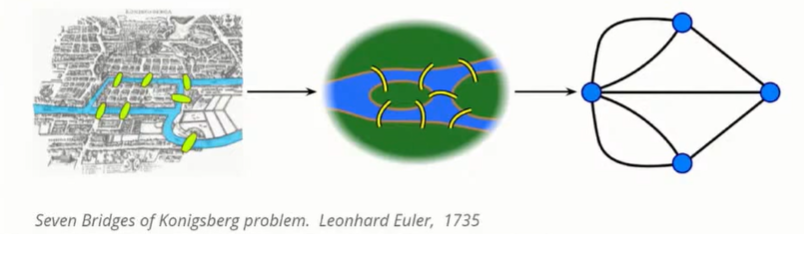
\includegraphics[width=\linewidth,keepaspectratio]{neo4j4}
\end{center}	  

Solution: No way!! What's the rule?

{\tiny (Ref: Introduction to Neo4j - a hands-on crash course - neo4j)}
\end{frame}


%%%%%%%%%%%%%%%%%%%%%%%%%%%%%%%%%%%%%%%%%%%%%%%%%%%%%%%%%%%
\begin{frame}[fragile]\frametitle{ Graph-structured Data Are Ubiquitous }

\begin{center}
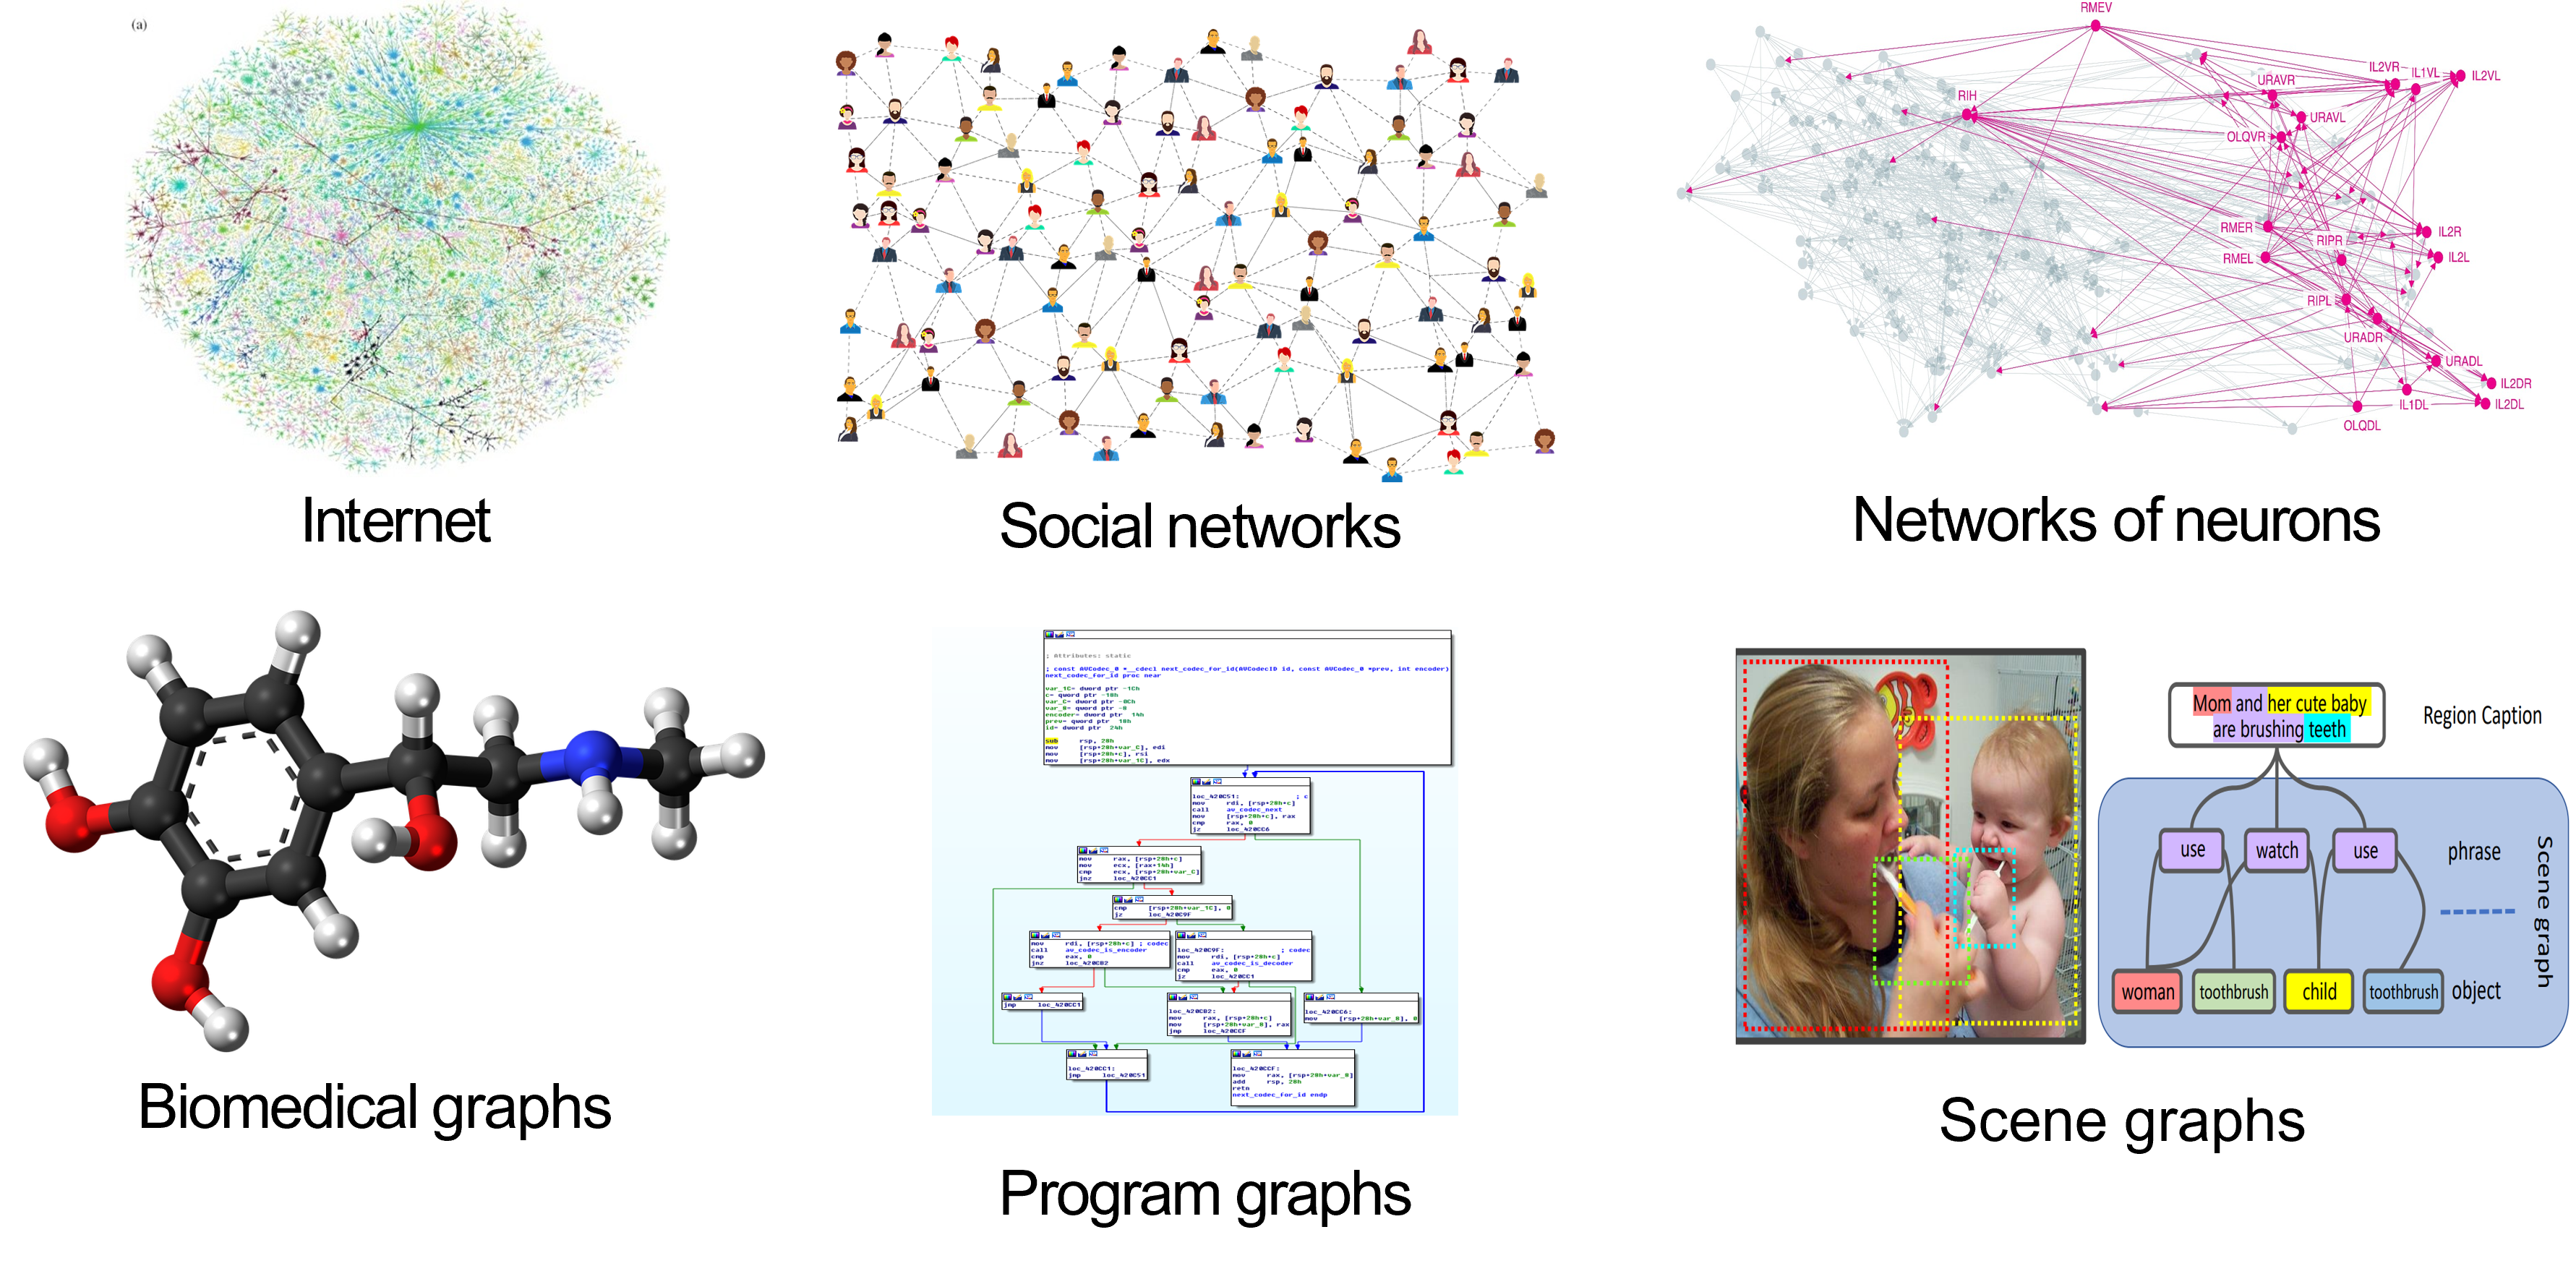
\includegraphics[width=\linewidth,keepaspectratio]{gnn1}
\end{center}	  

\end{frame}



%%%%%%%%%%%%%%%%%%%%%%%%%%%%%%%%%%%%%%%%%%%%%%%%%%%%%%%%%%%
\begin{frame}[fragile]\frametitle{Graphs: A Universal Language }

\begin{center}
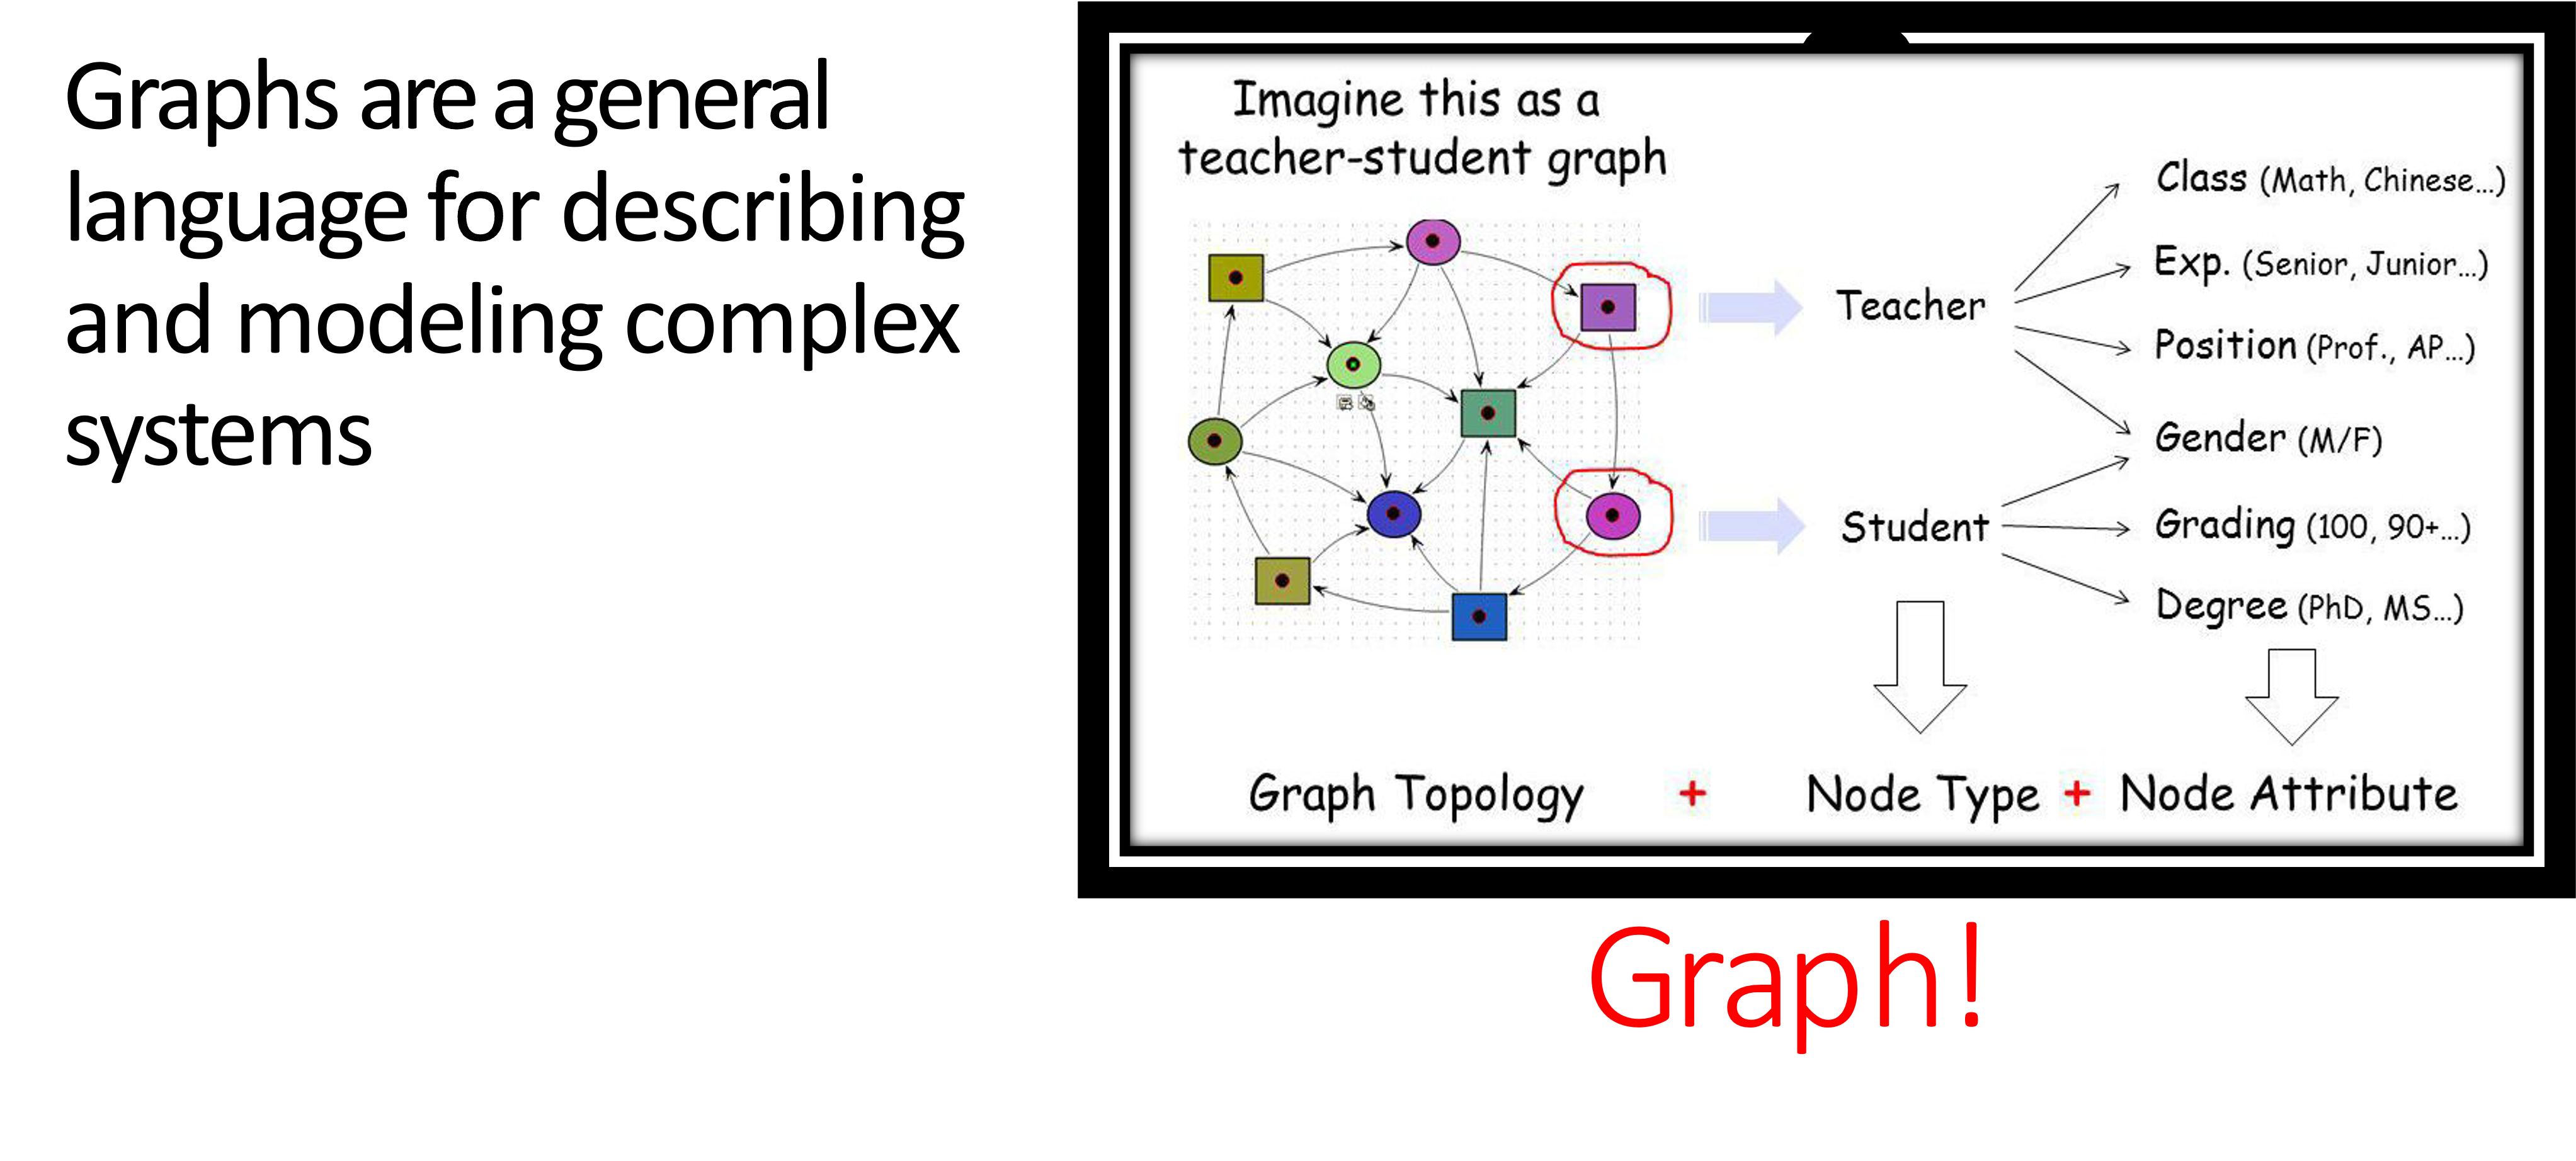
\includegraphics[width=\linewidth,keepaspectratio]{gnn4}
\end{center}	  

\end{frame}


%%%%%%%%%%%%%%%%%%%%%%%%%%%%%%%%%%%%%%%%%%%%%%%%%%%%%%%%%%%
\begin{frame}[fragile]\frametitle{Data as Graphs - Explicit }

\begin{center}
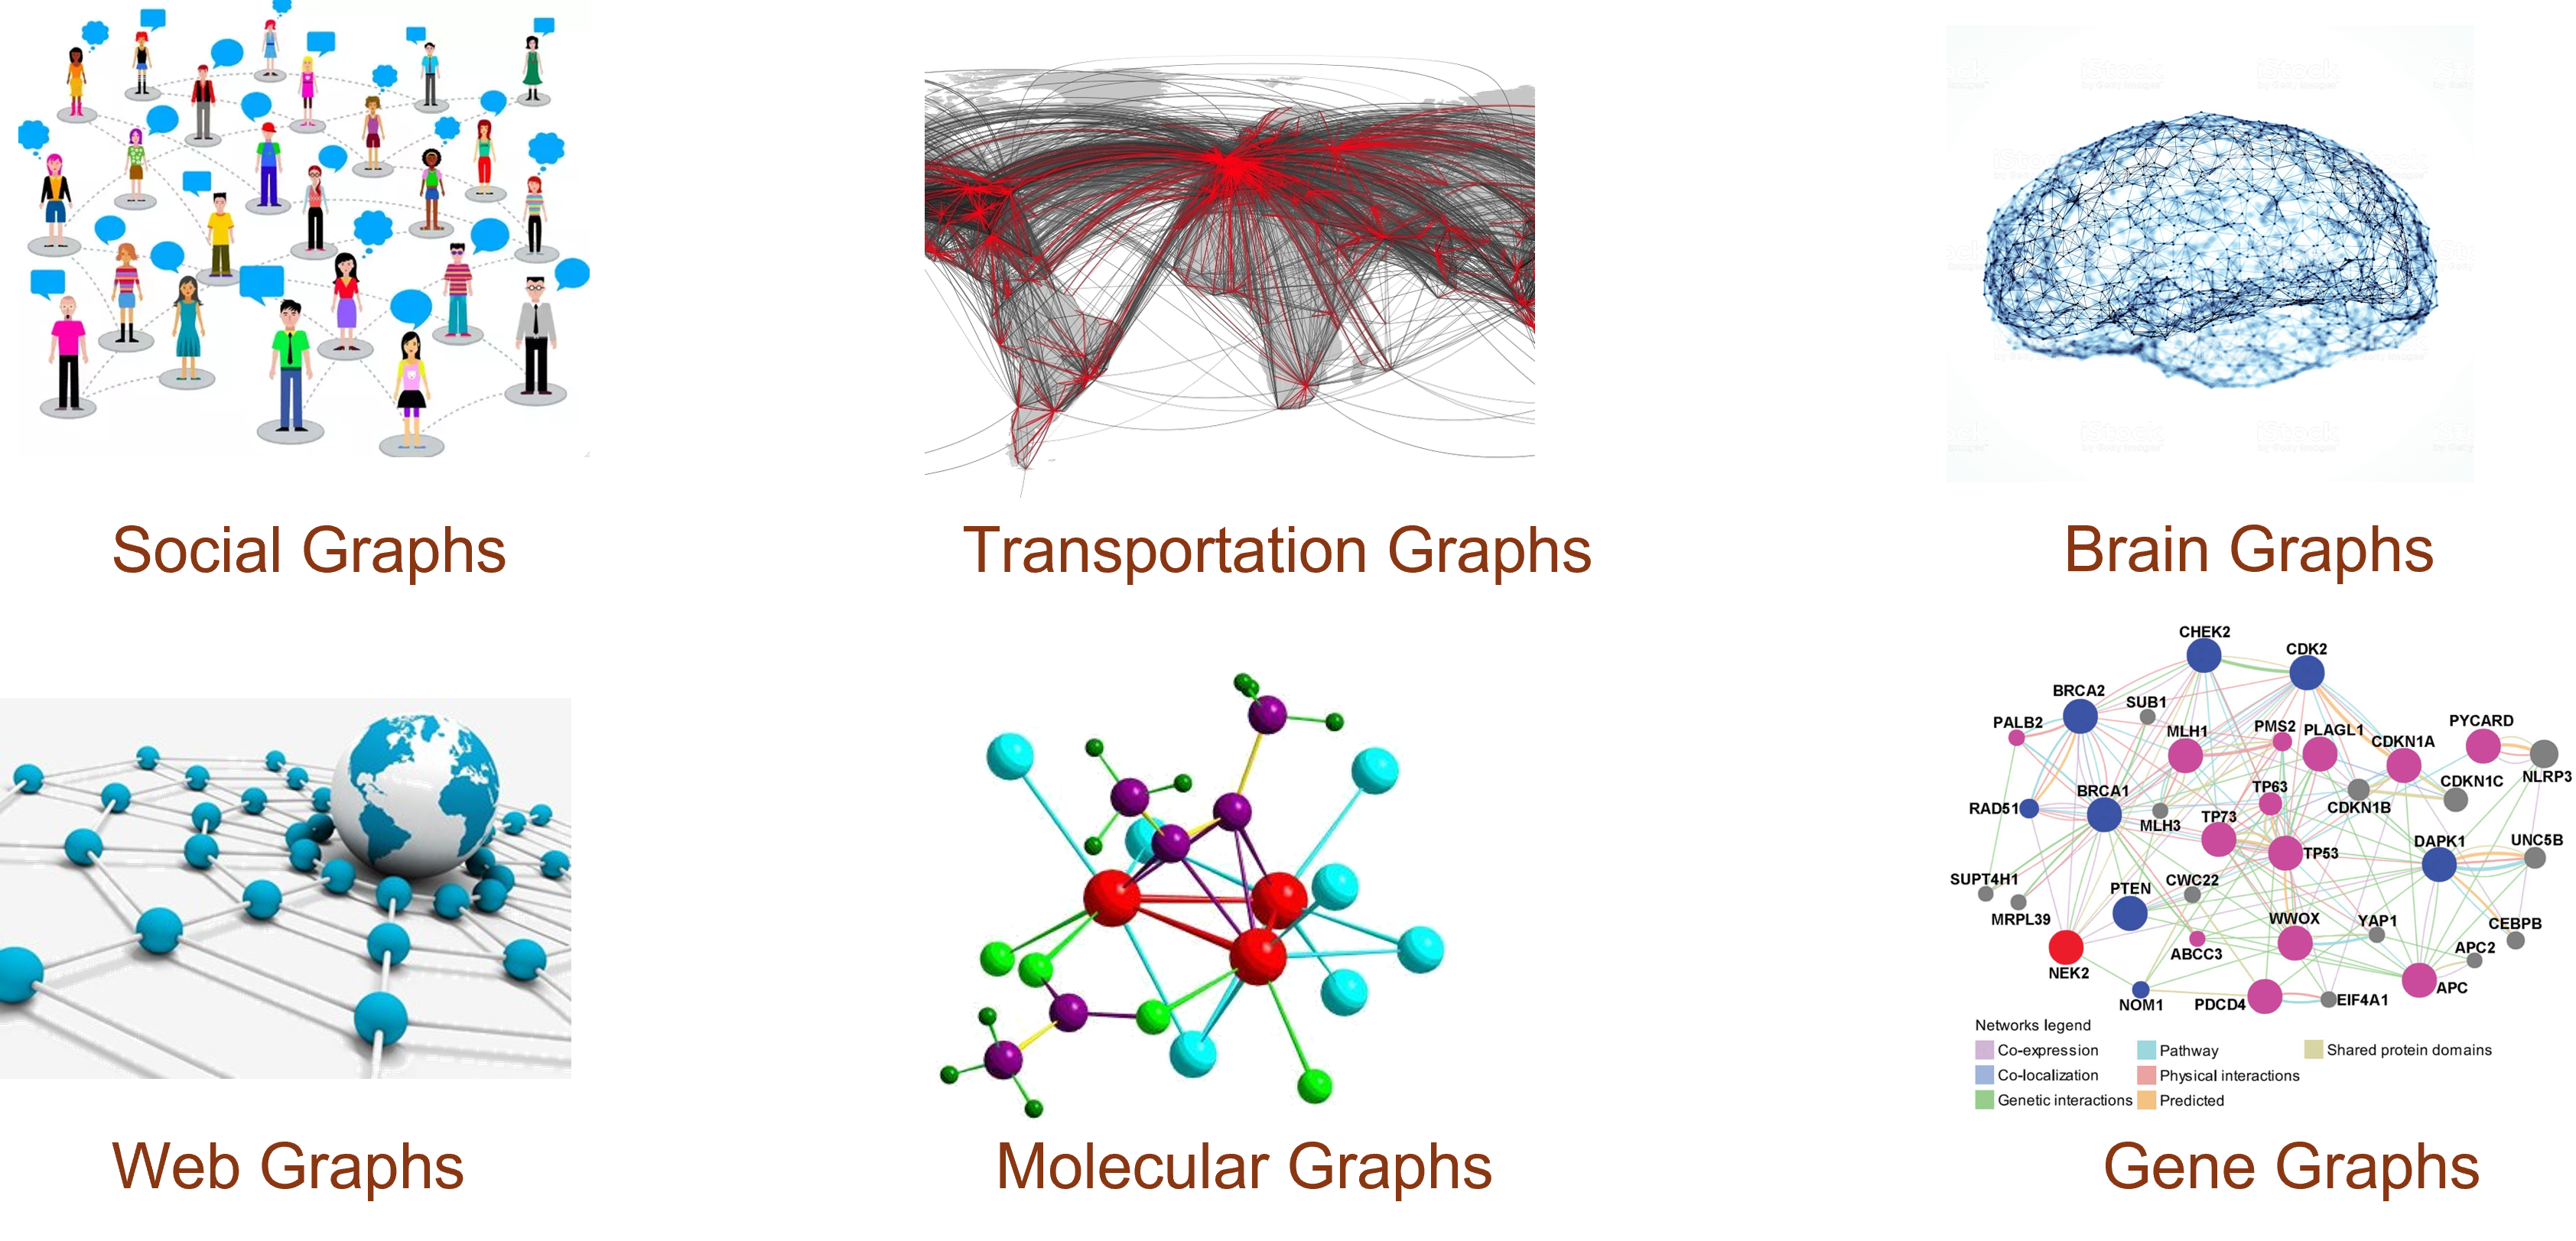
\includegraphics[width=\linewidth,keepaspectratio]{gnn5}
\end{center}	  

\end{frame}

%%%%%%%%%%%%%%%%%%%%%%%%%%%%%%%%%%%%%%%%%%%%%%%%%%%%%%%%%%%
\begin{frame}[fragile]\frametitle{Data as Graphs - Implicit }

\begin{center}
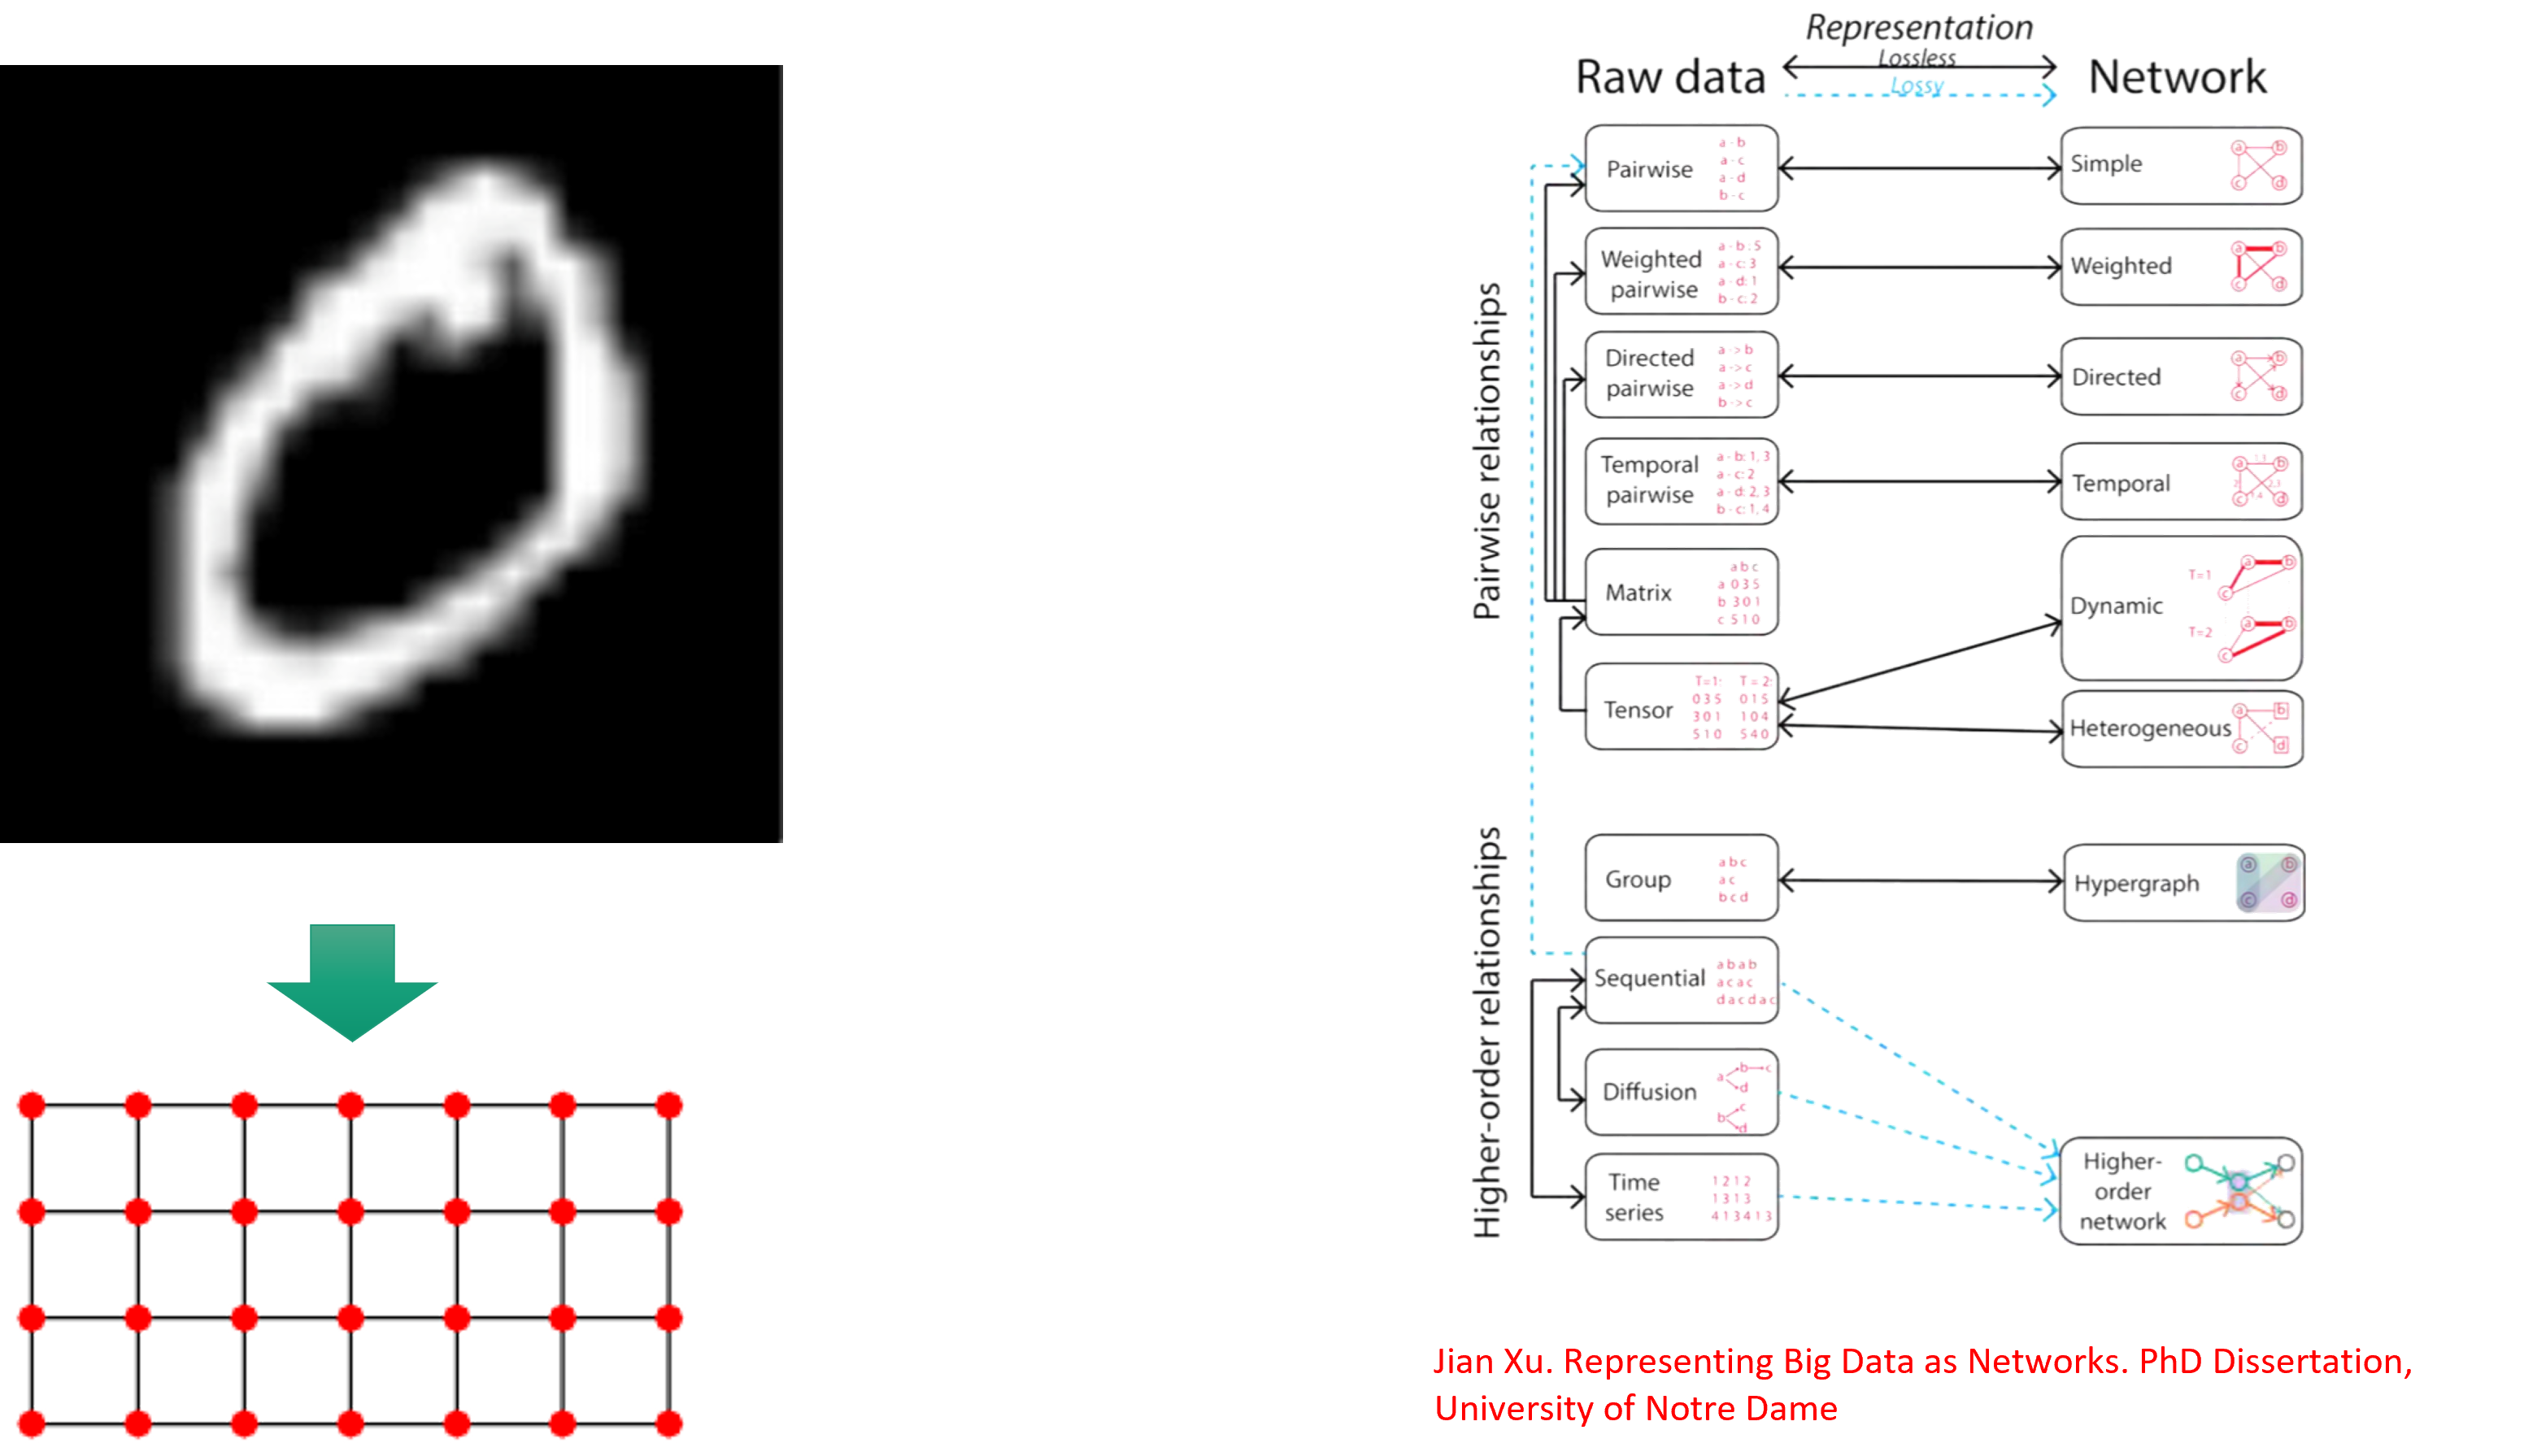
\includegraphics[width=\linewidth,keepaspectratio]{gnn6}
\end{center}	  

\end{frame}


%%%%%%%%%%%%%%%%%%%%%%%%%%%%%%%%%%%%%%%%%%%%%%%%%%%%%%%%%%%%%%%%%%%%%%%%%%%%%%%%%%
\begin{frame}\frametitle{ Graph Applications }

Across an organization, every department can benefit from graphs to answer questions 
like who or what is important, what should I do next, and what’s unusual about this?

\begin{center}
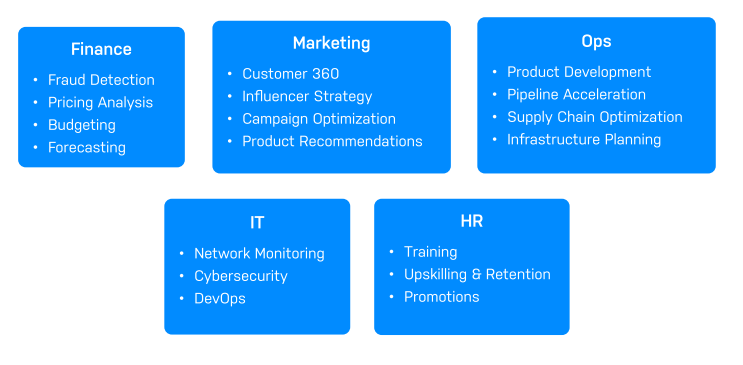
\includegraphics[width=\linewidth,keepaspectratio]{neo4j103}
\end{center}	  


{\tiny (Ref: 5 Graph Data Science Basics Everyone Should Know - neo4j)}
\end{frame}

%%%%%%%%%%%%%%%%%%%%%%%%%%%%%%%%%%%%%%%%%%%%%%%%%%%%%%%%%%%
\begin{frame}[fragile]\frametitle{A Knowledge Graph is}
 
\begin{center}
{\em \ldots an interconnected dataset enriched with meaning so we can reason about the underlying data and use it confidently for complex decision making}
\end{center}

	  - A neo4j definition
		
\end{frame}


%%%%%%%%%%%%%%%%%%%%%%%%%%%%%%%%%%%%%%%%%%%%%%%%%%%%%%%%%%%
\begin{frame}[fragile]\frametitle{A progression}
 
 of more enrichment \ldots
 
			\begin{center}
			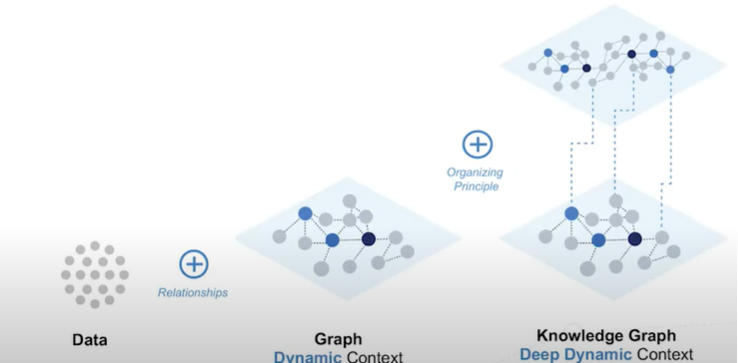
\includegraphics[width=\linewidth,keepaspectratio]{kg5}
			\end{center}	
			
			{\tiny (Ref: A Universe of Knowledge Graphs - neo4j)}
		
\end{frame}

%%%%%%%%%%%%%%%%%%%%%%%%%%%%%%%%%%%%%%%%%%%%%%%%%%%%%%%%%%%
\begin{frame}[fragile]\frametitle{Data}
 
 Variety of type/organization of data
 
			\begin{center}
			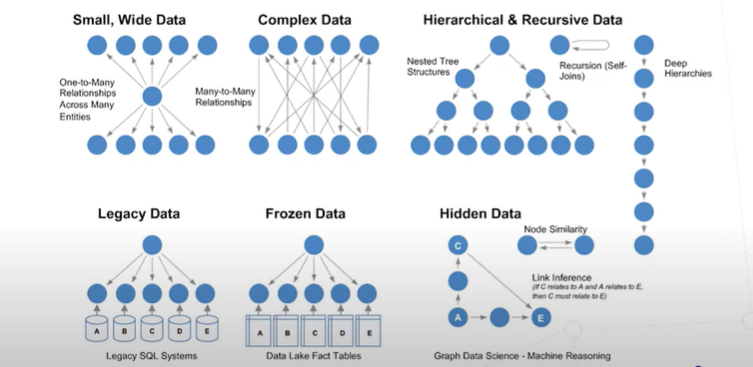
\includegraphics[width=\linewidth,keepaspectratio]{kg6}
			\end{center}	
			
			{\tiny (Ref: A Universe of Knowledge Graphs - neo4j)}
		
		
		``No more a Big Data but need Small and Wide data'' for more context in Machine Learning.
		
\end{frame}

%%%%%%%%%%%%%%%%%%%%%%%%%%%%%%%%%%%%%%%%%%%%%%%%%%%%%%%%%%%
\begin{frame}[fragile]\frametitle{Graphs}
 
 add Relationships to Data \ldots
 
 
			\begin{center}
			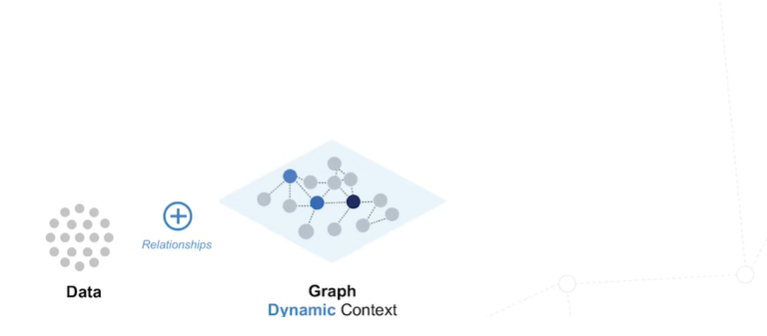
\includegraphics[width=\linewidth,keepaspectratio]{kg7}
			\end{center}	
			
			{\tiny (Ref: A Universe of Knowledge Graphs - neo4j)}
		
		
\end{frame}

%%%%%%%%%%%%%%%%%%%%%%%%%%%%%%%%%%%%%%%%%%%%%%%%%%%%%%%%%%%
\begin{frame}[fragile]\frametitle{Knowledge Graphs}
 
 add Organizing principles to Graphs \ldots
 
 
			\begin{center}
			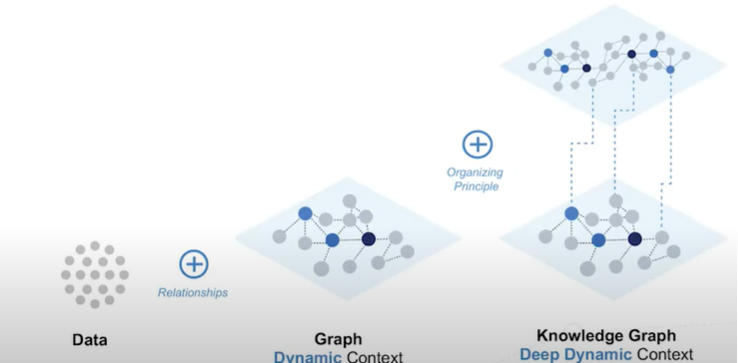
\includegraphics[width=\linewidth,keepaspectratio]{kg5}
			\end{center}	
			
			{\tiny (Ref: A Universe of Knowledge Graphs - neo4j)}
		
		e.g. external knowledge, ontologies injection. or 'Semantics'
		
\end{frame}


%%%%%%%%%%%%%%%%%%%%%%%%%%%%%%%%%%%%%%%%%%%%%%%%%%%%%%%%%%%
\begin{frame}[fragile]\frametitle{Semantics}
 
Semantics = Context = Domain Knowledge. 
 
			\begin{center}
			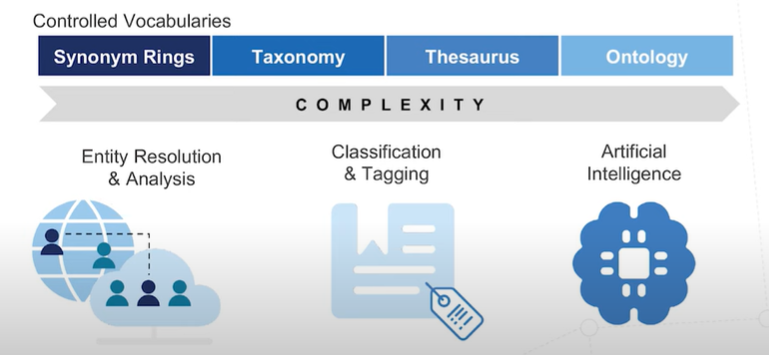
\includegraphics[width=\linewidth,keepaspectratio]{kg8}
			\end{center}	
			
			{\tiny (Ref: A Universe of Knowledge Graphs - neo4j)}
		
	
\end{frame}

%%%%%%%%%%%%%%%%%%%%%%%%%%%%%%%%%%%%%%%%%%%%%%%%%%%%%%%%%%%%%%%%%%%%%%%%%%%%%%%%%%
\begin{frame}\frametitle{So, a Knowledge Graph is}


\begin{columns}
    \begin{column}[T]{0.6\linewidth}

		Knowledge in Graph form.

			\begin{center}
			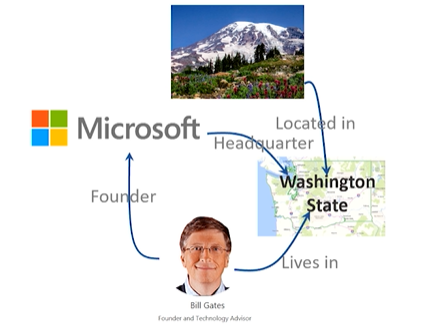
\includegraphics[width=\linewidth,keepaspectratio]{kg1}
			\end{center}	
    \end{column}
    \begin{column}[T]{0.4\linewidth}
			Embedded knowledge is:
			\begin{itemize}
			\item Microsoft is headquartered in Washington State.
			\item Bill Gates is a (co)Founder of Microsoft
			\item etc.
			\item Entities: Microsoft, Washington State, etc
			\item Relationships: founder, head, etc.
			\end{itemize}
    \end{column}
  \end{columns}
	

  

{\tiny (Ref: DAT278x - From Graph and Knowledge Graph - EdX course)}
\end{frame}


%%%%%%%%%%%%%%%%%%%%%%%%%%%%%%%%%%%%%%%%%%%%%%%%%%%%%%%%%%%%%%%%%%%%%%%%%%%%%%%%%%
\begin{frame}\frametitle{A Knowledge Graph is}

\begin{center}
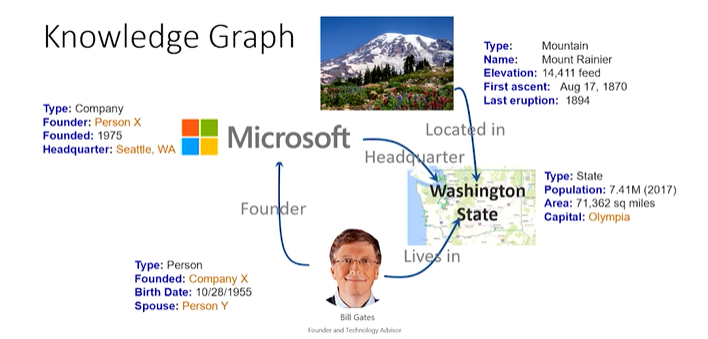
\includegraphics[width=\linewidth,keepaspectratio]{kg2}
\end{center}	

\begin{itemize}
\item Entities can be locations, companies, persons, etc. Nouns
\item Relationships can actions, has-a, etc. Verbs.
\end{itemize}


{\tiny (Ref: DAT278x - From Graph and Knowledge Graph - EdX course)}
\end{frame}

%%%%%%%%%%%%%%%%%%%%%%%%%%%%%%%%%%%%%%%%%%%%%%%%%%%%%%%%%%%%%%%%%%%%%%%%%%%%%%%%%%
\begin{frame}\frametitle{Knowledge Graph Datasets}

\begin{center}
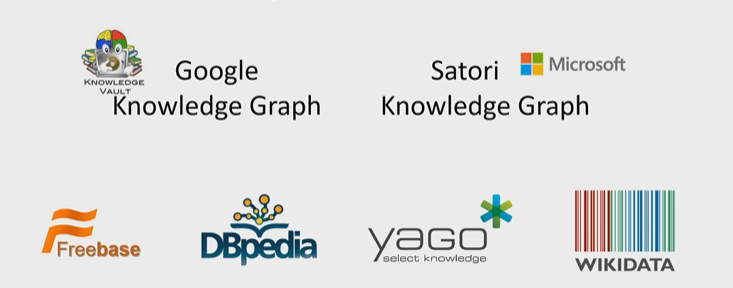
\includegraphics[width=\linewidth,keepaspectratio]{kg3}
\end{center}	

\begin{itemize}
\item Google, Microsoft KGs are private and used for search, question answering
\item DBPedia, Wikidata KGs are public
\end{itemize}

{\tiny (Ref: DAT278x - From Graph and Knowledge Graph - EdX course)}
\end{frame}

%%%%%%%%%%%%%%%%%%%%%%%%%%%%%%%%%%%%%%%%%%%%%%%%%%%%%%%%%%%%%%%%%%%%%%%%%%%%%%%%%%
\begin{frame}\frametitle{Domain specific Knowledge Graphs}

\begin{center}
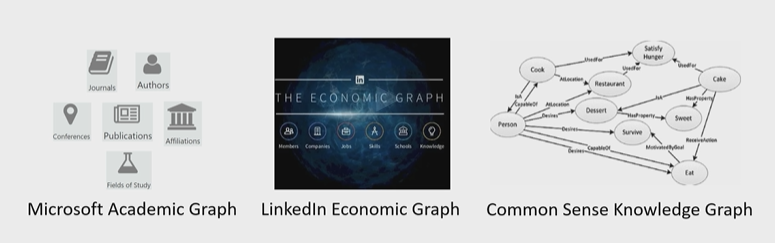
\includegraphics[width=\linewidth,keepaspectratio]{kg4}
\end{center}	


\begin{itemize}
\item Microsoft Academic Graph has 170 million papers and more than 200 million authors
\item LinkedIn Economic Graph has 500 million members and 20 million companies.
\end{itemize}

{\tiny (Ref: DAT278x - From Graph and Knowledge Graph - EdX course)}
\end{frame}


%%%%%%%%%%%%%%%%%%%%%%%%%%%%%%%%%%%%%%%%%%%%%%%%%%%%%%%%%%%%%%%%%%%%%%%%%%%%%%%%%%
\begin{frame}\frametitle{Why knowledge graph is important?}

\begin{itemize}
\item Help organize information
\item Tackle information overload
\item Intuitive explanation, visualization
\item Supports easy querying and business decisions.
\item Key component in many AI applications like Chatbot
\end{itemize}

{\tiny (Ref: DAT278x - From Graph and Knowledge Graph - EdX course)}
\end{frame}

%%%%%%%%%%%%%%%%%%%%%%%%%%%%%%%%%%%%%%%%%%%%%%%%%%%%%%%%%%%
\begin{frame}[fragile]\frametitle{Applications}
 
 
			\begin{center}
			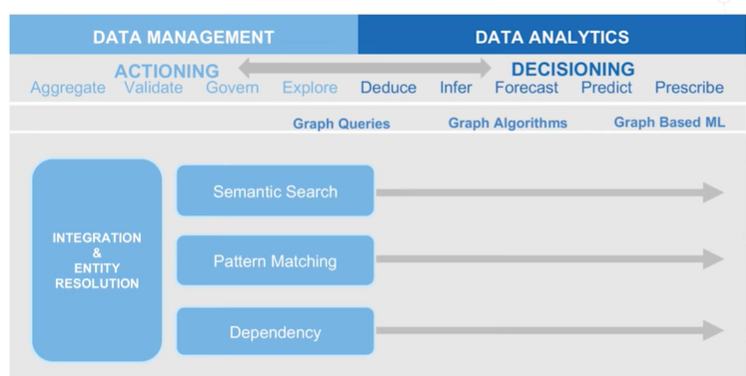
\includegraphics[width=\linewidth,keepaspectratio]{kg9}
			\end{center}	
			
			{\tiny (Ref: A Universe of Knowledge Graphs - neo4j)}
		
	
\end{frame}

%%%%%%%%%%%%%%%%%%%%%%%%%%%%%%%%%%%%%%%%%%%%%%%%%%%%%%%%%%%
\begin{frame}[fragile]\frametitle{Applications}
 
 Bridge data Silos
 
			\begin{center}
			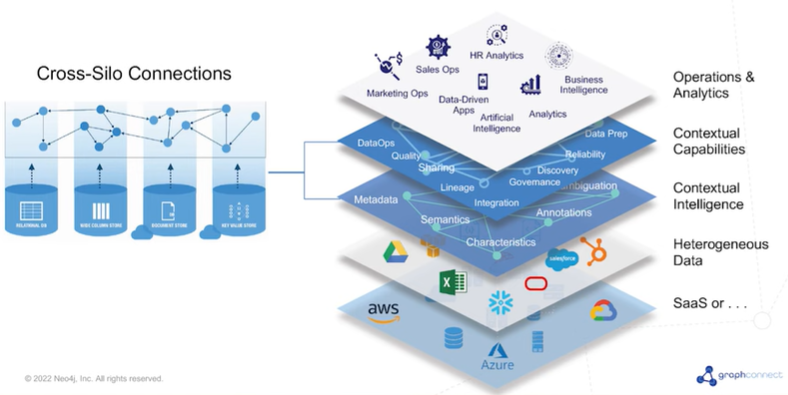
\includegraphics[width=\linewidth,keepaspectratio]{kg10}
			\end{center}	
			
			{\tiny (Ref: A Universe of Knowledge Graphs - neo4j)}
		
	
\end{frame}



%%%%%%%%%%%%%%%%%%%%%%%%%%%%%%%%%%%%%%%%%%%%%%%%%%%%%%%%%%%%%%%%%%%%%%%%%%%%%%%%%%
\begin{frame}\frametitle{Applications}

\begin{itemize}
\item Entity recommendation (Google right hand box): Searching via associated keywords
\item Semantic Search and recommendations using click logs
\item Personal Assistant like Alexa, Siri, using information associated with you.
\end{itemize}

{\tiny (Ref: DAT278x - From Graph and Knowledge Graph - EdX course)}
\end{frame}


%%%%%%%%%%%%%%%%%%%%%%%%%%%%%%%%%%%%%%%%%%%%%%%%%%%%%%%%%%%
\begin{frame}[fragile]\frametitle{Semantic Search}
 
 
			\begin{center}
			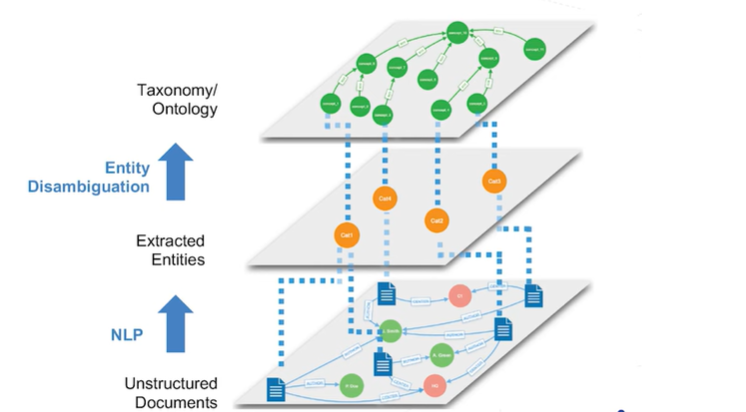
\includegraphics[width=\linewidth,keepaspectratio]{kg11}
			\end{center}	
			
			{\tiny (Ref: A Universe of Knowledge Graphs - neo4j)}
		
	
\end{frame}

%%%%%%%%%%%%%%%%%%%%%%%%%%%%%%%%%%%%%%%%%%%%%%%%%%%%%%%%%%%
\begin{frame}[fragile]\frametitle{Implicit Relationships}
 
	Candidate to Job matching via skills
 
			\begin{center}
			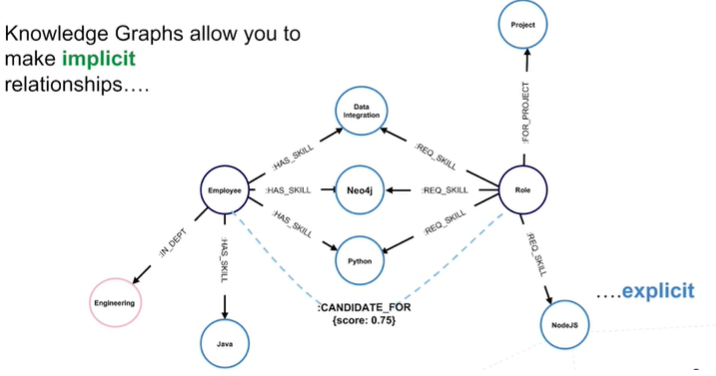
\includegraphics[width=\linewidth,keepaspectratio]{kg12}
			\end{center}	
			
			{\tiny (Ref: A Universe of Knowledge Graphs - neo4j)}
		
	
\end{frame}

%%%%%%%%%%%%%%%%%%%%%%%%%%%%%%%%%%%%%%%%%%%%%%%%%%%%%%%%%%%
\begin{frame}[fragile]\frametitle{Hidden Insights}
 
 
			\begin{center}
			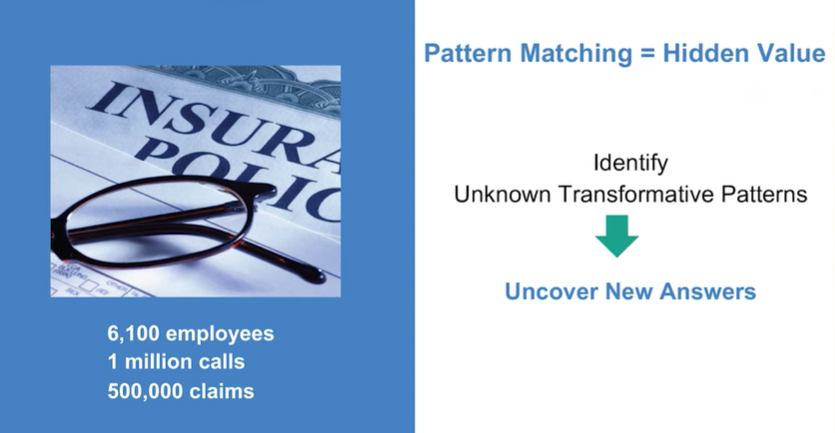
\includegraphics[width=\linewidth,keepaspectratio]{kg13}
			\end{center}	
			
			{\tiny (Ref: A Universe of Knowledge Graphs - neo4j)}
		
	
\end{frame}

%%%%%%%%%%%%%%%%%%%%%%%%%%%%%%%%%%%%%%%%%%%%%%%%%%%%%%%%%%%
\begin{frame}[fragile]\frametitle{Usages}
 
 
			\begin{center}
			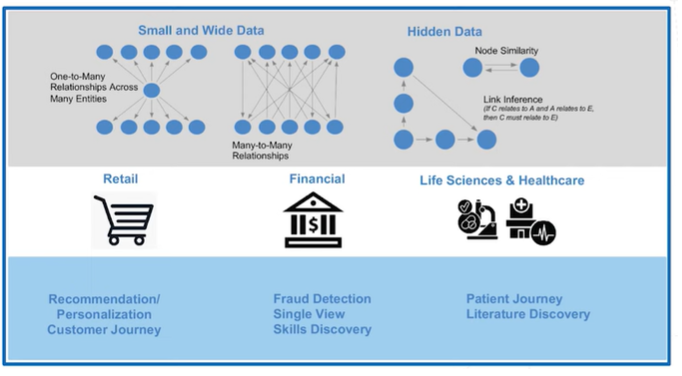
\includegraphics[width=\linewidth,keepaspectratio]{kg14}
			\end{center}	
			
			{\tiny (Ref: A Universe of Knowledge Graphs - neo4j)}
		
	
\end{frame}

%%%%%%%%%%%%%%%%%%%%%%%%%%%%%%%%%%%%%%%%%%%%%%%%%%%%%%%%%%%
\begin{frame}[fragile]\frametitle{Criticality}
 
 
			\begin{center}
			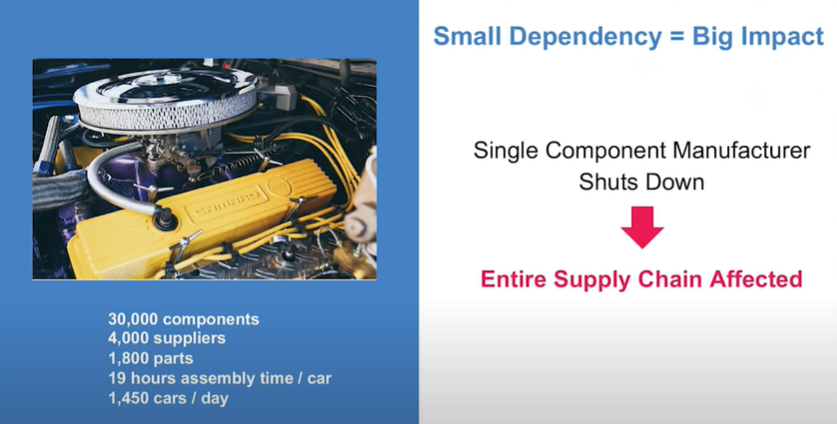
\includegraphics[width=\linewidth,keepaspectratio]{kg15}
			\end{center}	
			
			{\tiny (Ref: A Universe of Knowledge Graphs - neo4j)}
		
	
\end{frame}









%%%%%%%%%%%%%%%%%%%%%%%%%%%%%%%%%%%%%%%%%%%%%%%%%%%%%%%%%%%
\begin{frame}[fragile]\frametitle{References}

\begin{itemize}
\item DAT278x - From Graph and Knowledge Graph - EdX course
\item A Universe of Knowledge Graphs -  Dr. Maya Natarajan, Dr. Jesus Barrasa
\end{itemize}
	  
\end{frame}
















%%%%%%%%%%%%%%%%%%%%%%%%%%%%%%%%%%%%%%%%%%%%%%%%%%%%%%%%%%%
\begin{frame}[fragile]\frametitle{Sample Picture Inclusion}

\begin{center}
\includegraphics[width=0.8\linewidth,keepaspectratio]{myphoto}
\end{center}	  
\end{frame}

%%%%%%%%%%%%%%%%%%%%%%%%%%%%%%%%%%%%%%%%%%%%%%%%%%%
\begin{frame}[fragile] \frametitle{Sample Code Listing}
\begin{lstlisting}
import aaa
\end{lstlisting}

\end{frame}

%%%%%%%%%%%%%%%%%%%%%%%%%%%%%%%%%%%%%%%%%%%%%%%%%%%%%%%%%%%
\begin{frame}[fragile]\frametitle{Sample Two Columns Slide}
\begin{columns}
    \begin{column}[T]{0.6\linewidth}
      \begin{itemize}
		\item aaa
	  \end{itemize}

    \end{column}
    \begin{column}[T]{0.4\linewidth}
      \begin{itemize}
		\item bbb
	  \end{itemize}
    \end{column}
  \end{columns}
\end{frame}

%%%%%%%%%%%%%%%%%%%%%%%%%%%%%%%%%%%%%%%%%%%%%%%%%%%%%%%%%%%%%%%%%%%%%%%%%%%%%%%%%%%
\begin{frame}[fragile]\frametitle{Sample Tabular Data}

aaa

\begin{tabular}{|c|c|}
	\hline
	Platform & Time (s) \\
	\hline \hline
	Python & $\sim$1500.0 \\
	\hline
	NumPy & 29.3 \\
	\hline
	Matlab & $\sim$29.0 \\
	\hline
	Octave & $\sim$60.0 \\
	\hline
	Blitz (C++) & 9.5 \\
	\hline
	Fortran & 2.5 \\
	\hline
	C & 2.2 \\
	\hline
\end{tabular}

\end{frame}
